\chapter{The Limits of Direct Reinforcement Learning of Decision Tree Policies}
In this chapter we investigate the properties of reinforcement learning for learning a depth-1 decision tree policy for a very simple Markov decision process.
Using the formal framework of partially observable iterative bounding Markvov decision processes (cite), we aim to learn partially observable deterministic policies that correspond to decision tree policies (cite).

We will attempt to learn a depth-1 tree policy for the $2\times 2$ grid world from (cite) as the base MDP by soving the example POIBMDP from the previous chapter.
To focus on reinforcement learning properties in POIBMDPs rather than, e.g., modelling properties, we will carefully craft POIBMDPs such that the \textit{optimal} partially observable deterministic policy corresponds to a depth-1 tre policy.
To do so, we present next how the POIBMDP objective values (cite) from different decision tree policies change with $\zeta$ for some fixed discount factor $\gamma$.  

\section{Constructing POIBMDPs which optimal solutions are the depth-1 tree}
\begin{figure}[htbp]
    \centering
    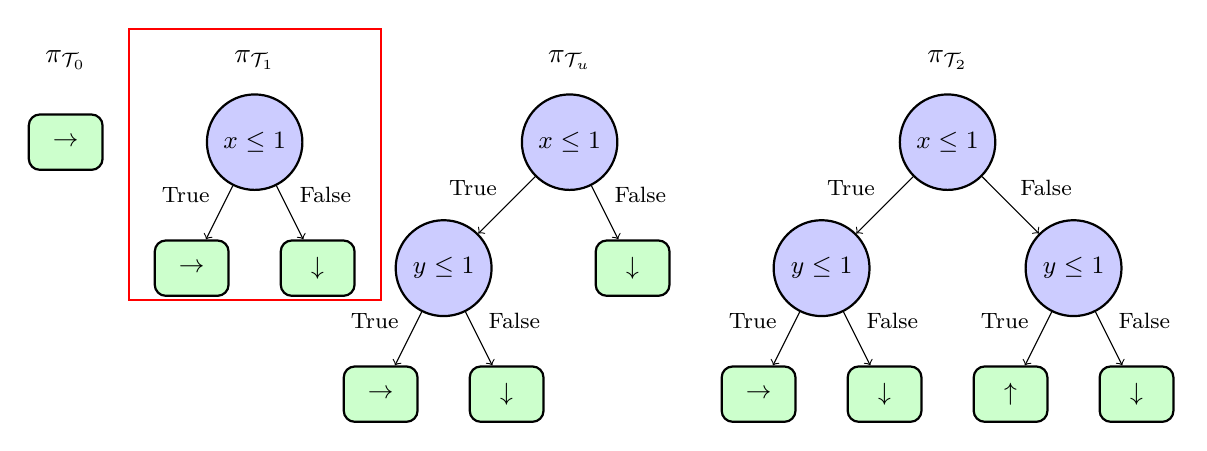
\begin{tikzpicture}[
        scale=0.8,
        decision/.style={circle, draw, thick, fill=blue!20, text width=2.5em, text centered, minimum height=2.5em, font=\small},
        leaf/.style={rectangle, draw, thick, fill=green!20, text width=2em, text centered, rounded corners, minimum height=2em, font=\small},
        edge_label/.style={font=\footnotesize, midway}
    ]
        
        \node[leaf] at (-3, 0) {$\rightarrow$};
        % Tree 4: if x <= 0.5 move right else move left
        \node[decision] (tree4_root) at (0,0) {$x \leq 1$};
        \node[leaf] (tree4_right) at (-1,-2) {$\rightarrow$};
        \node[leaf] (tree4_left) at (1,-2) {$\downarrow$};
        \draw[->] (tree4_root) -- (tree4_right) node[edge_label, above left] {True};
        \draw[->] (tree4_root) -- (tree4_left) node[edge_label, above right] {False};
        
        % Draw a square around the tree
        \draw[thick, red] (-2, 1.8) rectangle (2, -2.5);

        % Tree 7: if x <= 0.5 and y <= 0.5 move right else move down
        \node[decision] (tree7_root) at (5,0) {$x \leq 1$};
        \node[decision] (tree7_y) at (3,-2) {$y \leq 1$};
        \node[leaf] (tree7_right) at (2,-4) {$\rightarrow$};
        \node[leaf] (tree7_down) at (4,-4) {$\downarrow$};
        \node[leaf] (tree7_down2) at (6,-2) {$\downarrow$};
        \draw[->] (tree7_root) -- (tree7_y) node[edge_label, above left] {True};
        \draw[->] (tree7_root) -- (tree7_down2) node[edge_label, above right] {False};
        \draw[->] (tree7_y) -- (tree7_right) node[edge_label, above left] {True};
        \draw[->] (tree7_y) -- (tree7_down) node[edge_label, above right] {False};


        \node[decision] (tree7_root) at (11,0) {$x \leq 1$};
        \node[decision] (tree7_y) at (9,-2) {$y \leq 1$};
        \node[decision] (tree7_y2) at (13,-2) {$y \leq 1$};
        \node[leaf] (tree7_right) at (8,-4) {$\rightarrow$};
        \node[leaf] (tree7_down) at (10,-4) {$\downarrow$};
        \node[leaf] (tree7_right2) at (12,-4) {$\uparrow$};
        \node[leaf] (tree7_down2) at (14,-4) {$\downarrow$};
        \draw[->] (tree7_root) -- (tree7_y) node[edge_label, above left] {True};
        \draw[->] (tree7_root) -- (tree7_y2) node[edge_label, above right] {False};
        \draw[->] (tree7_y) -- (tree7_right) node[edge_label, above left] {True};
        \draw[->] (tree7_y) -- (tree7_down) node[edge_label, above right] {False};
        \draw[->] (tree7_y2) -- (tree7_right2) node[edge_label, above left] {True};
        \draw[->] (tree7_y2) -- (tree7_down2) node[edge_label, above right] {False};

        % Labels
        \node[above] at (-3,1) {$\pi_{\mathcal{T}_0}$};
        \node[above] at (0,1) {$\pi_{\mathcal{T}_1}$};
        \node[above] at (5,1) {$\pi_{\mathcal{T}_u}$};
        \node[above] at (11,1) {$\pi_{\mathcal{T}_2}$};


    \end{tikzpicture}
    \caption{For each decision tree structure, e.g., depth-1 or unbalanced depth-2, in the space of deterministic partially observable POIBMDP policies, we illustrate the decision tree which gets the highest base rewards.}
    \label{fig:optimal-policy-trees}
\end{figure}

In this section we compute the \textit{exact} objective values of the POIBMDP policies and look for $\zeta$ values such that the optimal POIBMDP policy corresponds to a depth-1 decision tree for the grid world MDP like the one in Figure (cite).  
Indeed, because we know all the base states, all the observations, all the actions, all the rewards and all the transitions, we can compute exactly the values of different partially observable deterministic policies given $\zeta$ the reward for IGAs and $\gamma$ the discount factor.

Each of those policies can be one of the following trees illustrated Figure (cite): 
\begin{itemize}
    \item a depth-0 tree equivalent to always taking the same base action 
    \item a depth-1 tree equivalent alternating between an IGA and a base action 
    \item an unbalanced depth-2 tree that sometimes takes two IGAs then a base action and sometimes a an IGA then a base action
    \item a depth-2 tree that alternates between taking two IGAs and a base action
    \item an inifinite ``tree'' that only takes IGAs
\end{itemize}
Furthermore, because from (cite) we know that for POMDPs stochastic policies can sometimes be optimal we also compute the value of the stochastic policy that alternates between two base actions.

We detail the calculations for the detpth-1 decision tree objective value (cite) and defer the calculations for the other policies to the Appendix (cite).

\begin{proposition}[Depth-1 decision tree objective value] The objective value of the best depth-1 decision tree from Figure (cite) is $V^{\pi_{\mathcal{T}_1}}(o_0) = \frac{4\zeta + \gamma + 2\gamma^3 + \gamma^5}{4(1-\gamma^2)}$.
\end{proposition}

\begin{proof} $\pi_{\mathcal{T}_1}$ has one root node that tests $x\leq1$ (respectively $y\leq1$) and two leaf nodes $\rightarrow$ and $\downarrow$. 
To compute $V^\pi_{\mathcal{T}_1}(o_0)$, we compute the values of $\pi_{\mathcal{T}_1}$ in each of the possible startin states $(s_0, o_0), (s_1, o_0), (s_2, o_0), (s_g, o_0)$ and compute the expectation over those. 
At inititalization, when the base state is $s_g = (1.5, 0.5)$, the depth-1 decision tree policy cycles between taking an information gathering action $x\leq1$ and moving down to get a positive reward for which it gets the returns:
\begin{align*}
    V^{\pi_{\mathcal{T}_1}} (s_g, o_0) &= \zeta + \gamma + \gamma^2 \zeta + \gamma^3 \dots \\
    &= \overset{\infty}{\underset{t=0}\sum} \gamma^{2t} \zeta + \overset{\infty}{\underset{t=0}\sum} \gamma^{2t+1} \\
    &= \frac{\zeta + \gamma}{1 - \gamma^2}
\end{align*}
At inititialization, in either of the base states $s_0=(0.5,0.5)$ and $s_2=(1.5, 1.5)$, the value of the depth-1 decision tree policy is the return when taking one information gathering action $x\leq1$, then moving right or down, then following the policy from the goal state $s_g$:
\begin{align*}
    V^{\pi_{\mathcal{T}_1}} (s_0, o_0) &= \zeta + \gamma 0 + \gamma^2 V^{\pi_{\mathcal{T}_1}} (s_g, o_0) \\
    &= \zeta + \gamma^2 V^{\pi_{\mathcal{T}_1}} (s_g, o_0) \\
    &= V^{\pi_{\mathcal{T}_1}} (s_2, o_0)
\end{align*}
Similarly, the value of the best depth-1 decision tree policy in state $s_1=(0.5,1.5)$ is the value of taking one information gathering action then moving right to $s_2$ then following the policy in $s_2$:
\begin{align*}
    V^{\pi_{\mathcal{T}_1}} (s_1, o_0) &= \zeta + \gamma 0 + \gamma^2 V^{\pi_{\mathcal{T}_1}} (s_2, o_0) \\
    &= \zeta + \gamma^2 V^{\pi_{\mathcal{T}_1}} (s_2, o_0) \\
    &= \zeta + \gamma^2 (\zeta + \gamma^2 V^{\pi_{\mathcal{T}_1}} (s_g, o_0)) \\
    &= \zeta + \gamma^2 \zeta + \gamma^4 V^{\pi_{\mathcal{T}_1}} (s_g, o_0)
\end{align*}
Since the probability of being in any base states at initialization given that the agent observe $o_0$ is the probability of being in any base states at initialization, we can write:
\begin{align*}
    V^{\pi_{\mathcal{T}_1}} (o_0) &= \frac{1}{4} V^{\pi_{\mathcal{T}_1}} (s_g, o_0) + \frac{2}{4} V^{\pi_{\mathcal{T}_1}} (s_2, o_0) + \frac{1}{4} V^{\pi_{\mathcal{T}_1}} (s_1, o_0) \\
    &= \frac{1}{4} \frac{\zeta + \gamma}{1 - \gamma^2} + \frac{2}{4} (\zeta + \gamma^2 \frac{\zeta + \gamma}{1 - \gamma^2}) + \frac{1}{4} (\zeta + \gamma^2 \zeta + \gamma^4 \frac{\zeta + \gamma}{1 - \gamma^2}) \\
    &= \frac{1}{4} \frac{\zeta + \gamma}{1 - \gamma^2} + \frac{2}{4} (\frac{\zeta + \gamma ^ 3}{1-\gamma^2}) + \frac{1}{4}(\frac{\zeta+\gamma^5}{1-\gamma^2}) \\
    &= \frac{4\zeta + \gamma + 2\gamma^3 + \gamma^5}{4(1-\gamma^2)}
\end{align*}
\end{proof}


\begin{figure}
    \centering
    \includegraphics[width=1\textwidth]{images/images_part1/objective_values_plot.pdf}
    \caption{POIBMDP objective values of different policies as functions of $\zeta$. Shaded areas show the optimal policies in different ranges of $\zeta$ values.}\label{fig:objectives}
\end{figure}

We can now plot the POIBMDP objective values of the different policies corresponding to trees for the grid world MDP as function of $\zetas$ when we fix $\gamma=0.99$. 
When $\gamma=0.99$, despite objective values being very similar for the depth-1 and unbalanced depth-2 tree, we now know that {\color{blue}a depth-1 tree is the optimal deterministic partially observable POIBMDP policy for $0< \zeta < 1$}.

Interestingly, two challenges from POMDPs can already be observed from Figure (cite). 
First, there is a whole range of $\zeta$ values for which the stochastic policy is optimal.
Second, for e.g. $\zeta=0.5$, when the depth-1 tree is the optimal deterministic partially observable policy, the value of state $(s_2, o_0) = (1.5, 1.5, 0, 2, 0, 2)$ is not maximized by the optimal policy but by the policy that always goes down which is sub-optimal.
Next, we use reinforcement learning to obtain POIBMDP policies corresponding to trees for the grid world MDP.

\section{Results}

Now that we have shown theoretically that there exists values of $zeta$ such that the depth-1 tree policy from Figure (cite) is optimal in terms of IBMDP value (cite) and is also optimal in terms of MDP value (cite),
we show that existing algorithms fail to learn the depth-1 tree even though it is the optimal IBMDP policy.
We conjecture that this is because learning decision tree policies in IBMDP is equivalent to learning a deterministic reactive POMDP policy.

\subsection{Experimental Setup}
\paragraph{IBMDP:} we will benchmark RL algorithms for the IBMDP of Section (cite) when the base part of the state is hidden to guarantee that the learned policy is a tree.
There are two information gathering actions $x\leq0.5$ and $y\leq0.5$.
We have to be extra careful when implementing this grid world because we work in the setting of discounted infinite horizon MDP; so in theory trajectories are infinite which is prohibited in practice.
To ensure that trajectories are diverse, we reset the learning agent every 100 steps in the MDP.
Furthermore we try to solve 200 different IBMDPs. Each IBMDP has $\gamma$ fixed to 0.99 and $\zeta$ value linearly spaced in $[-1, 2]$.
\paragraph{Baselines:} we consider two groups of RL algorithms. The first group is standard tabular RL; Q-learning (cite)(cite), Sarsa (cite)(cite), and Policy Gradient (cite)(cite).
(cite) and (cite) already studied the theoritcal and practical implications of applying standard RL directly to POMDP by considering partial observations as full states.
(cite) proved that Q-Learning will converge but without optimality guarantees. 
(cite) showed empirically that Sarsa-$\lambda$ (cite), a version of Sarsa with some sort of memory, can learn good deterministic solutions to POMDP.
We draw similar conclusions from our experiments. 
We also use a vanilla tabular Policy Gradient baseline (cite), which to the best of our knowledge, nobody studied in our setting.
In theory PG should not be a good candidate algorithm to solve our problem since it can learn stochastic policies that we showed can be better than our target policy (cite).


More recently, new algorithms were developped specially for our setting of learning policies for POMDPs. Those algorithms are called asymmetric RL which authors of (cite) use without knowing. 
Asymmetric algorithms, also called (rememebr name deployment); leverage the fact that, even if the deployed policy should depend only on partial observation, nothing forbids the use of full state information during training.
Asymmetric Q-learning (cite) make use of state-dependent Q function $Q:S\timesA \rightarrow \mathbb{R}$ to use a TD target to update a $Q:O\times A\rightarrow \mathbb{R}$ (cite)(algo).    
Asymmetric Policy Gradient (cite) use a state-dependent critic $V:S\rightarrow \mathbb{R}$ to plug into the gradient estimate of a policy $\pi:O\times A \rightarrow \mathbb{R}$.
We benchmark Asymmetric Q-learning and Asymmetric Sarsa and the tabular algorithm from (cite) that we call JSJ in our experiments (algo) which is equivalent to a tabular Asymmetric Policy Gradient.
In previous work (cite) Deep RL version of asymmetric algorithms have been benchmarked and showed to only work well for history-dependent policies or Q-function which we can't use for our particular problem.
In particular in Figures (cite)(cite) of (cite) and cite(); the authors show that for the particular case of asymmetric critic or target depending on full states and policy or Q-function depending on partial observation, the performance of asymmetric RL can be worse than that of non-specialized naive RL.
We use at least one million timesteps to train each agent. Each agent is trained on 100 seeds.  

\RestyleAlgo{ruled}
\SetKwComment{Comment}{}{}
\begin{algorithm}
    \KwData{POMDP $\mathcal{M}_{po} = \langle X, O, A, R, T, T_0, \Omega \rangle$, learning rates $\alpha_1,\quad \alpha_2$, exploration rate $\epsilon$}
    \KwResult{Partially observable deterministic policy $\pi$}
    Initialize $U(x,a) = 0$ for all $x \in X, a \in A$ \\
    Initialize $Q(o,a) = 0$ for all $o \in O, a \in A$ \\

    \For{each episode}{
        Initialize state $x_0 \sim T_0$ \\
        Initialize observation $o_0 \sim \Omega(x_0)$ \\

        \For{each step $t$}{
            Choose action $a_t$ using $\epsilon$-greedy: $a_t = \arg\max_a Q(o_t,a)$ with prob. $1-\epsilon$ \\
            Take action $a_t$, observe $r_t = R(x_t,a_t)$, $x_{t+1} \sim T(x_t,a_t)$, and $o_{t+1} \sim \Omega(x_{t+1})$ \\
            $y \leftarrow r + \gamma U(x_{t+1}, \argmax_{a'} Q(o_{t+1}, a'))$ \Comment{// TD target} \\
            $U(x_t,a_t) \leftarrow (1 - \alpha_1) U(x_t, a_t) + \alpha_1 y $ \\
            $Q(o_t,a_t) \leftarrow (1 - \alpha_1) Q(o_t, a_t) + \alpha_1 y $ \\
            $x_t \leftarrow x_{t+1}$ \\
            $o_t \leftarrow o_{t+1}$ \\
        }
    }
    $\pi(o) = \arg\max_a Q(o,a)$ \Comment{// Extract greedy policy}
    \caption{Asymmetric Q-Learning (cite)}\label{alg:asymqlearning}
\end{algorithm}

\RestyleAlgo{ruled}
\SetKwComment{Comment}{}{}
\begin{algorithm}
    \KwData{POMDP $\mathcal{M}_{po} = \langle X, O, A, R, T, T_0, \Omega \rangle$, learning rate $\alpha$, policy parameters $\theta$, number of trajectories $N$}
    \KwResult{Policy $\pi_\theta$ and Q-function estimates}
    Initialize policy parameters $\theta$ \\
    Initialize $Q(o, a) = 0$ for all observations $o$ and actions $a$ \\
    \For{each episode}{
        \For{$i = 1$ to $N$}{
            Generate trajectory $\tau_i = (s_0, a_0, r_0, s_1, a_1, r_1, \ldots, s_T)$ following $\pi_\theta$ \\
            \For{each timestep $t$ in trajectory $\tau_i$}{
                $G_t \leftarrow \sum_{k=t}^{T} \gamma^{k-t} r_k$ \Comment{// Compute return}
                Store $(o_t, a_t, G_t)$ for later averaging
            }
        }
        \For{each unique observation-action pair $(o, a)$}{
            $Q(o, a) \leftarrow \frac{1}{|\{(o, a)\}|} \sum_{(o, a, G)} G$ \Comment{// Monte Carlo estimate}
        }
        \For{each observation $o$}{
            \For{each action $a$}{
                $\pi_1(a|o) \leftarrow 1.0$ if $a = \argmax_{a'} Q(o, a')$, $0.0$ otherwise \Comment{// Deterministic policy from Q-values}
                $\pi(a|o) \leftarrow (1 - \alpha) \pi(a|o) + \alpha \pi_1(a|o)$ \Comment{// Policy improvement step}
            }
        }
        Reset $Q(o, a) = 0$ for all observations $o$ and actions $a$ \Comment{// Reset for next episode}
    }
    \caption{JSJ algorithm. Uses Monte Carlo estimates of the average reawrd value functions to perform policy imporvements (cite)}\label{alg:reinforce}
\end{algorithm}

\paragraph{Hyperparameters:} For all RL baselines in the first part of this section we use, when applicable, exploration rates $\epsilon=0.3$ and/or learning rates $\alpha=0.1$.

\paragraph{Metrics:} we will consider two main metrics; the sub-optimality gap of the learned policy with respect to the IBMDP objective (cite) and the proportion of the type of learned decision tree for the original grid world.
Because we know the whole (IB)MDP model that we can represent exactly as tables; and because we know for each $\zeta$ value the IBMDP objective value of the optimal partially observable IBMDP policy; we can report the \textbf{exact} sub-optimality gaps:
\begin{align*}
    \operatorname{Gap}(\pi) = |V(\pi^{\star}) - V(\pi)|
\end{align*}
Where we can compute $V(\pi)$ exactly by first mapping $\pi : O \times A \rightarrow \mathbb{R}$ to $\pi_{S} : S \times A \rightarrow \mathbb{R}$ by setting $\pi_S (s, a) = \pi(o,a) \text{ if }o\in s$ $\forall s \in S, \forall o \in O \forall a \in A$.
And then we apply repetitevly the Bellman operator (show).
Similarly, once the RL training finished, we can use the tree extraction algorithm (cite) to count the learned tree distributions across the 100 seeds of each experiment.

\subsection{How well do exsisting baselines learn in POIBMDPs?}

\begin{figure}
    \centering
    \includegraphics[width=1\textwidth]{images/images_part1/learning_curves.pdf}
    \caption{Baseline algorithms for learning decision tree policies by learning partially observable policies in IBMDPs. 
    The top row represents the sub-optimality gaps during training. In each subplot, each single learning curve is colored by the value of $\zeta$ of the IBMDP they solve. And each single learning curve represent the sub-optimality gap averaged over 100 seeds.
    So for each algortihm we ran a total of $200 \times 100$ single training seed.
    The bottom row represents the distributions of final tree policies learned across the 100 seeds.
    For each $\zeta$ value, there are three color points each represeting the share of Depth-0 tree (red), Depth-1 tree (gree) and Depth-2 tree (blue).
    }\label{fig:rl-poibmdp}
\end{figure}

\begin{figure}
    \centering
    \includegraphics[width=1\textwidth]{images/images_part1/tree_distributions.pdf}
    \caption{Baseline algorithms for learning decision tree policies by learning partially observable policies in IBMDPs. 
    The top row represents the sub-optimality gaps during training. In each subplot, each single learning curve is colored by the value of $\zeta$ of the IBMDP they solve. And each single learning curve represent the sub-optimality gap averaged over 100 seeds.
    So for each algortihm we ran a total of $200 \times 100$ single training seed.
    The bottom row represents the distributions of final tree policies learned across the 100 seeds.
    For each $\zeta$ value, there are three color points each represeting the share of Depth-0 tree (red), Depth-1 tree (gree) and Depth-2 tree (blue).
    }\label{fig:dt-distrib-poibmdp}
\end{figure}

In Figure (cite) we observe that despite RL algorithms converging independently of the $\zeta$ values, not all runs fully minimize the sub-optimality gap.
In particular all RL algorithms properly minimze the gap, i.e. learn the optimal policy or Q-function, for $\zeta \in [-1, 0]$, where the optimal policy is to repeat going right or down,
Similarly all RL algorithms properly learn the optimal solutions for $\zeta \in [1, 2]$, where the optimal policy is to repeat taking informathion gathering actions. 
While in $\zeta \in ]0, 1[$ where the depth-1 tree is optimal, no baseline can learn the optimal solution. 
In this range, baselines also converge to trees deeper than 1.
One interpretation of this phenomenon is that the learning in POIBMDPs is very hard and so agents tend to converge to easy policies: repeating the same actions (whether it is a base or an information gathering action). 


\subsection{Why is it so hard to learn in POIBMPDs?}

\begin{table}[h]
\centering
\caption{Sarsa Hyperparameter Space (48 combinations)}
\begin{tabular}{lll}
\toprule
\textbf{Hyperparameter} & \textbf{Values} & \textbf{Description} \\
\midrule
Epsilon Start & 0.1, 0.3, 1.0 & Initial exploration rate \\
Epsilon Decay & 0.99, 0.999, 1.0 & Exploration rate decay \\
Lambda & 0.0, 0.3, 0.6, 0.9 & Eligibility trace decay \\
Learning Rate (lr\_o) & 0.001, 0.005, 0.01, 0.1 & Observation SARSA learning rate \\
Optimistic & True, False & Optimistic initialization \\
\bottomrule
\end{tabular}
\end{table}

\begin{table}[h]
\centering
\caption{SARSA-Asym Hyperparameter Space (192 combinations)}
\begin{tabular}{lll}
\toprule
\textbf{Hyperparameter} & \textbf{Values} & \textbf{Description} \\
\midrule
Epsilon Start & 0.1, 0.3, 1.0 & Initial exploration rate \\
Epsilon Decay & 0.99, 0.999, 1.0 & Exploration rate decay \\
Lambda & 0.0, 0.3, 0.6, 0.9 & Eligibility trace decay \\
Learning Rate (lr\_1) & 0.001, 0.005, 0.01, 0.1 & $Q$ learning rate \\
Learning Rate (lr\_2) & 0.001, 0.005, 0.01, 0.1 & $U$ learning rate \\
Optimistic & True, False & Optimistic initialization \\
\bottomrule
\end{tabular}
\end{table}

\begin{table}[h]
    \centering
    \caption{Summary of All Algorithm Hyperparameter Spaces (780 total combinations)}
    \begin{tabular}{llr}
    \toprule
    \textbf{Algorithm} & \textbf{Problem} & \textbf{Total Hyperparameter Combinations} \\
    \midrule
    Policy Gradient & POIBMDP & 140 \\
    Policy Gradient & IBMDP & 140 \\
    Q-learning & POIBMDP &48 \\
    Asym Q-learning & POIBMDP & 192 \\
    Q-Learning & IBMDP & 60 \\
    Sarsa & POIBMDP & 48 \\
    Asym Sarsa & POIBMDP & 192 \\
    Sarsa & IBMDP & 60 \\
    \bottomrule
    \end{tabular}
    \end{table}

As discussed in the previous chapter (cite), POIBMDPs inherit many difficulties from POMDPs (list).
To prove that solving POIBMDPs even though there are only a handful of states and observations and clear deterministic reactive optimal policies; we compare the success rate of baselines RL algorithms when applied to an IBMDP with $\gamma=0.99$, $\zeta=0.5$, and to the partially observable version of the same IBMDP.
because we know that for those values of $\zeta$ and $\gamma$, the optimal partially observable policy is the depth-1 tree and the optimal-fully observable policy is the (cite); we can compute the success rate of an RL algorithm as the proportion of learn policies that match either optimal policy.
In particular, for each of the three baselines Q-Learning, Sarsa, and Policy gradient, and their asymmetric counterparts when available; we train policies with each combination of those hyperparameters (cite) 10 times and compute the success rate over all individual runs.
To fully quantify the difficulty of RL on those problems; we also consider advanced tricks for tabular RL.
\begin{enumerate}
    \item Optimistic Q-function (cite)
    \item Entropy regularization (cite)
    \item Eligibility traces (cite)
    \item $\epsilon$-decay (cite)
\end{enumerate}

\begin{figure}
    \centering
    \includegraphics[width=1\textwidth]{images/images_part1/algorithm_performance_comparison_flattened.pdf}
    \caption{Success rates of different RL algorithms over thousands of runs on two variants of the same IBMDP; the default and Partially observable one.}\label{fig:po-vs-ib}
\end{figure}

The key observations from Figure (cite) is that POIBMDPs are way harder than their IBMDPs counterparts.
Even though asymmetry seems to increase performance; learning a decision tree policy for a simple grid world directly with RL seem way to difficult and costly.
We suggest researcher and practitioners interested in decision tree policies to forget the direct RL approach and focus on the indirect imitation-based approach (cite).
Or, if for some reason one needs to still use reinforcement learning training; fitting parametric trees, trees whose depth and nodes are predifined and where only thresholds are optimized, then one can use SYMPOL (cite) or Soft decision trees (cite).

In the next chapter, we show that when the base MDP's transitions are independent of the action, then POIBMDPs are actually \textit{fully} observable.